%%%% ijcai11.tex

\typeout{IJCAI Switching Planner Submission}

% These are the instructions for authors for IJCAI-11.
% They are the same as the ones for IJCAI-07 with superficical wording
%   changes only.

\documentclass{article}
% The file ijcai11.sty is the style file for IJCAI-11 (same as ijcai07.sty).
\usepackage{ijcai11}

% Use the postscript times font!
\usepackage{times}

% the following package is optional:
%\usepackage{latexsym} 

% Following comment is from ijcai97-submit.tex:
% The preparation of these files was supported by Schlumberger Palo Alto
% Research, AT\&T Bell Laboratories, and Morgan Kaufmann Publishers.
% Shirley Jowell, of Morgan Kaufmann Publishers, and Peter F.
% Patel-Schneider, of AT\&T Bell Laboratories collaborated on their
% preparation.

% These instructions can be modified and used in other conferences as long
% as credit to the authors and supporting agencies is retained, this notice
% is not changed, and further modification or reuse is not restricted.
% Neither Shirley Jowell nor Peter F. Patel-Schneider can be listed as
% contacts for providing assistance without their prior permission.

% To use for other conferences, change references to files and the
% conference appropriate and use other authors, contacts, publishers, and
% organizations.
% Also change the deadline and address for returning papers and the length and
% page charge instructions.
% Put where the files are available in the appropriate places.



\usepackage{subfig}
\usepackage{tikz}
\usetikzlibrary{shapes}
\usetikzlibrary{positioning}

\usepackage{graphicx}
\graphicspath{{plots/}}

\newcommand{\solver}[1]{{\sc #1}}
\newcommand{\system}[1]{\solver{#1}}
\newcommand{\problem}[1]{{\rm #1}}
\newcommand{\pcogx}{\solver{PCogX}}


\newcommand{\actNam}[1]{\texttt{#1}}
\newcommand{\pp}[1]{\actNam{#1}}

\newcommand{\Expect}{\makebox[1em]{$\mathbin{\mbox{\sf E}}$}}

\newtheorem{definition}{Definition}
\newtheorem{proposition}{Proposition}
\newtheorem{lemma}{Lemma}
\newtheorem{theorem}{Theorem}
\newtheorem{property}{Property}
\newtheorem{corollary}{Corollary}

\newcommand{\laostar}{\textsc{lao$^*$}}
\newcommand{\fastdownward}{\textsc{FastDownward}}


\newcommand{\obsDist}{\ensuremath{\mathit{v}}}

\newcommand{\states}{\ensuremath{\mathcal{S}}}
\newcommand{\state}{\ensuremath{s}}
\newcommand{\observ}{\ensuremath{o}}
\newcommand{\observation}{\ensuremath{\observ}}
%% \newcommand{\percept}{\ensuremath{\widetilde{\observ}}}
\newcommand{\reward}{\ensuremath{{\sf R}}}
\newcommand{\transProb}{\ensuremath{{\sf Pr}}}
%% \newcommand{\States}{\ensuremath{\mathbb{S}}}
%% \newcommand{\TransProb}{\ensuremath{\textbf{Pr}}}
%% \newcommand{\Reward}{\ensuremath{\reward}}
%% \newcommand{\Actions}{\ensuremath{\mathbb{A}}}
%% \newcommand{\Observ}{\ensuremath{\mathbb{O}}}
\newcommand{\observations}{\ensuremath{O}}
\newcommand{\policy}{\ensuremath{\pi}}
\newcommand{\actions}{\ensuremath{\mathcal{A}}}
\newcommand{\action}{\ensuremath{a}}

%% \newcommand{\object}{\ensuremath{o}}
%% \newcommand{\objects}{\ensuremath{\mathcal{O}}}

\newcommand{\bstate}{\ensuremath{b}}

\newcommand{\Omit}[1]{}

\newcommand{\props}{\ensuremath{{\cal P}}}
\newcommand{\prop}{\ensuremath{p}}
\newcommand{\propositions}{\props}
\newcommand{\percepts}{\ensuremath{\Pi}}
\newcommand{\percept}{\ensuremath{\pi}}

\newcommand{\stochActions}{\ensuremath{\actions}}
\newcommand{\detActions}{\ensuremath{\actions^d}}
\newcommand{\stochAction}{\ensuremath{\action}}
\newcommand{\detAction}{\ensuremath{\action^d}}
\newcommand{\stochAct}{\stochAction}
\newcommand{\detAct}{\detAction}

\newcommand{\stochSenses}{\ensuremath{K}}
\newcommand{\detSenses}{\ensuremath{K^d}}
\newcommand{\stochSense}{\ensuremath{\kappa}}
\newcommand{\detSense}{\ensuremath{\kappa^d}}


\newcommand{\poss}{\ensuremath{\pp{poss}}}
\newcommand{\add}{\ensuremath{\pp{ add}}}
\newcommand{\delete}{\ensuremath{\pp{delete}}}



\newcommand{\nodes}{\ensuremath{\mathcal{N}}}
\newcommand{\selections}{\ensuremath{\Psi}}
\newcommand{\transitions}{\ensuremath{\Eta}}
\newcommand{\node}{\ensuremath{n}}
\newcommand{\selection}{\ensuremath{\psi}}
\newcommand{\transition}{\ensuremath{\eta}}


\def\oom{$^{\tt +}$}
\def\zom{$^*$}
\def\bump{\hspace{1cm}}
\newenvironment{tabtt}{\begin{tt}\begin{tabbing}}{\end{tabbing}\end{tt}}%

%% \title{Interleaved Serial and Decision-Theoretic Planning for a Mobile Robot}

\title{Interleaved Serial and Decision-Theoretic Planning for
Practical Robot Control}

%% \title{A Switching Planner for Combined Task and Observation Planning}
\author{anonymous}

\begin{document}

\maketitle

\begin{abstract}

%% Those processes must 

From an automated planning perspective the problem of practical mobile
robot control in realistic environments poses many important and
contrary challenges.  On the one hand, the planning process must be
lightweight, robust, and timely. Over the lifetime of the robot it
must always respond quickly with new plans that accommodate exogenous
events, changing objectives, and the underlying unpredictability of
the environment.  On the other hand, in order to exhibit useful
behaviours the planning process must perform computationally expensive
reasoning about contingencies and possible revisions of subjective
beliefs according to quantitatively modelled uncertainty in acting and
sensing.
%%
Towards addressing these challenges, we develop a \emph{continual
planning} approach that {\em switches} between using a fast
satisficing ``classical'' planner, to decide on the overall strategy,
and decision-theoretic planning to solve small subproblems where
deeper consideration of the sensing model is both practical, and can
significantly impact overall performance. We demonstrate our approach
in large problems from a realistic robot exploration domain.

%% partial observability



%% In cooperation with execution monitoring, it must perform repair
%% and/or replanning in order to seamlessly accommodate exogenous events,
%% changing objectives, and the underlying unpredictability of the
%% environment.

%% Realistic robot planning problems in uncertain environments often
%% require achieving tasks while also finding out about the
%% world. Because the world state cannot be observed directly, these
%% problems are naturally represented as partially observable Markov
%% decision problems (POMDPs). However, these are typically intractable
%% for realistic problems.
%%


\end{abstract}

\section{Introduction}

Planning for agents acting in partially observable environments with
stochastic actions is extremely computationally
expensive~\cite{mdp-complexity}. Even relatively small partially
observable Markov decision problems (POMDPs), represented by tens of
propositional variables, have state spaces far larger than existing
optimal or close to optimal planners can handle. For the easier
problem of planning in completely observable stochastic domains, an
alternative has been to use classical sequential planners and
replan when actions have unplanned-for outcomes~\cite{yoon:etal:2007}.
Execution monitoring tracks properties of the state that determine
whether further planning is required. For partially observable
domains, only probabilistic information about such properties will, in
general, be available.

%% However, these approaches rely
%% crucially on being able to determine properties of the current state
%% in order to decide to replan. For partially observable domains, only
%% probabilistic information about these properties will in general be
%% available.

This paper describes the planning component for a robotic system that
continuously deliberates in a stochastic dynamic environment in order
to achieve objectives set by the user, and acquire knowledge about its
surroundings. This domain features partial observability, particularly
because the state is not perfectly known, and state information is
gained by the robot through the use of unreliable sensing
actions. 
%Using a propositionally factored state representation, for
For
interesting sized tasks the corresponding POMDP model is too large for a
POMDP solver to be applied directly. Inspired by the replanning
approaches used successfully for MDP
planning~\cite{yoon:etal:2007,yoon:etal:2008}, we propose a continual
planning approach that uses a classical planning system to compute a
reasonably valuable trace in the model, and then uses a
decision-theoretic planner on small subproblems where reasoning about
observations might be useful. We refer to the complete system as a
{\em switching continual planner}. The approach is not optimal,
particularly as it relies on the results of sequential planning
directly. It does nevertheless perform better than a purely sequential
replanner, and is fast enough to be used for real-time decision-making
on a mobile robot.


%% Switching gives us some important advantages in our robotic
%% domain. First, the significant source of uncertainty in the domain is
%% the unreliability of observations, and this approach is particularly
%% suited to problems that combine a deterministic task planning problem
%% with observations as the decision-theoretic planner is often invoked
%% to determine a characteristic of the underlying state. Secondly,
%% replanning makes our system robust to changing objectives and the
%% discovery of new facts about the world.


%% As an illustration, consider a robot searching for a box that it knows
%% is often found in offices. The sequential planner might produce a plan
%% that assumes that {\sc Room a} is an office, that the box is in {\sc
%% Room a}, and that the box is in location 1 in {\sc Room a}. Given
%% these assumptions, the plan might be to go to {\sc Room a}, go to
%% location 1 and search for the box. When the plan gets executed and the
%% search begins the decision-theoretic planner is called since searching
%% involves making observations. The decision-theoretic planner might
%% retract the last assumption but leave the others, and build a plan to
%% search the whole of {\sc Room a} for the box. If this plan fails to
%% find the box, it will disprove the assumption that the box is in {\sc
%% Room a}, which will then lead to replanning by the sequential planner
%% based on the newly discovered knowledge.

Our system is domain independent, taking domain and problem
descriptions in a first-order declarative language we have developed,
called the decision-theoretic planning domain definition language
(DTPDDL). From these descriptions of POMDPs, we automatically
construct a deterministic model suitable for sequential planners. That
model includes actions which correspond to making assumptions about
the values of imperfectly known state variables. Assumptions scheduled
by the sequential system are used to propose a pragmatic abstract
belief-state space to the decision-theoretic system, and to modify the
reward function, so that system might pursue sensing related to those
assumptions.

%%  which can operate
%% with the original representation of the domain.


%% The sequential planner we use is based
%% on \fastdownward~\cite{fast-downward}. We add the capability to replan
%% ~\cite{brenner:nebel:jaamas09}, and also allow agent
%% knowledge to be represented explicitly, so we can write actions that
%% gain the agent knowledge. LEASE CITE MICHAEL's WORK AS THE BASIS FOR
%% THIS. For the decision-theoretic planner we have implemented our own
%% forward search in the belief-state space.


The switching planner provides important advantages in our
mobile robot domain. First, the significant source of uncertainty in the
domain is the unreliability of observations and this approach is
particularly suited to problems that combine a deterministic task
planning problem with observations because the decision-theoretic planner
is only invoked to deal with state uncertainty.
%determine a characteristic of the underlying state. 
Secondly, replanning makes the system robust to
changing objectives and discoveries about the world,
both of which feature in our domain.

The remainder of the paper proceeds as follows. We begin by describing
POMDPs with a propositionally factored representation of states and
observations. We also outline the relationship between this and a flat
POMDP representation. Next we describe our DTPDDL language with
example declarations from a mobile robot exploration task. Then we
describe the switching planner, including how the sequential domain is
produced and a plan is generated, and how this then provides the input
for the decision-theoretic planner. Finally we provide an evaluation
of the system on the example robot domain, and finish with a short
survey of related work and some concluding remarks.





%To accompany
%that language we have implemented an information-state
%\laostar\ procedure for solving problems expressed in DTPDDL. 

%%

%Have a good understanding of the contents and function of rooms, as
%well as the linguistic referrents to rooms, widgets, and their visual
%qualities.

%Having confidence in its beliefs about the linguistic terms for
%spaces, and the function of those spaces.



%sometimes difficult to predict, with exogenous events, such as the
%changing of the objective, 





%the speed and scalability of software for sequential planning in
%deterministic




%% We developed a first-order declarative language, called DTPDDL, for
%% describing domains of planning problems that correspond to POMDPs.  To
%% accompany that language we have implemented an information-state
%% \laostar\ procedure for solving problems expressed in DTPDDL. 

%% We have extended MAPSIM to parse and simulate DTPDDL problems, and
%% modified \fastdownward\ so that it can find useful sequential executions
%% given DTPDDL models of the problem at hand.




%%  called DTPDDL, along
%% the lines of PDDL for the partially observable case, an \laostar\
%% solution procedure, a determinisation of the DTPDDL problem in MAPL,
%% and modify the \fastdownward\ system to find high quality sequential plans
%% .

%% We model the environment as a partially observable Markov decision
%% process. Although planning in that model is undecidable in
%% general~\cite{}, an optimal finite-horizon plan corresponds to a
%% contingent plan, that is a function mapping action-observation
%% histories to actions.

%% our continual planner is reactive, replanning whenever the underlying
%% domain and problem models change. For example, replanning occurs if
%% the motivational component alters the objectives, and if an assumed
%% outcome of a sensing action is not realised.

%% brittle sensing model, 

%% the evaluation of a fluent at a state is either known. Moreover, there
%% is a sensing process that run-time variables  after-which 

%% For $\prop \in \state$ we say proposition $\prop$ characterises state
%% $\state$. There is always a unique starting state $\state_0$. The goal
%% $\goal$ is a set of propositions, and we say that state $\state$ is a
%% goal state iff $\goal \subseteq \state$.

%%  To keep this exposition
%% simple, for any two distinct actions $\stochAction_i \neq
%% \stochAction_j$, if outcome $\detAct$ is a possibility for
%% $\stochAction_i$ then it cannot also be a possibility for
%% $\stochAction_j$ -- i.e., if $\detAct \in
%% \detActions(\stochAction_i)$ then $\detAct \not\in
%% \detActions(\stochAction_j)$.


%% The solution to a probabilistic planning problem is a contingency
%% plan. This consists of an assignment of actions to states at each
%% discrete timestep up to the planning horizon $n$. The optimal
%% contingency plan is one which prescribes actions to states that
%% maximise the probability that the goal is achieved within $n$ steps
%% from the starting state $\state_0$. For the purposes of this paper
%% we say a plan fails, i.e. achieves the goal with probability $0$, in
%% situations where it does not prescribe an action. Computing the
%% optimal plan for a problem is computationally intractable, and an
%% important direction for research in the field is to develop
%% heuristic mechanisms for generating small linear plans
%% quickly~\cite{littman:etal:98}



\section{Propositional Decision-Theoretic Planning}

%% {\em runtime variables}
%% {\em decision variables}
%% {\em uninitialised variables}
%% {\em omitted variables}

We describe the partially observable propositional probabilistic
planning problem, with costs and rewards. We model a process state
$\state$ as the set of propositions that are true of the
state. Notationally, $\props$ is the set of propositions, $\prop$ is
an element from that set, and we have $\state \subseteq
\props$. The underlying process
dynamics are modelled in terms of a finite set of {\em probabilistic
STRIPS operators}~\cite{boutilier:abstraction} $\stochActions$ over
state-characterising propositions $\propositions$.
%%
We say an action $\stochAction \in \stochActions$ is
applicable if its precondition $\poss(\stochAction)$, a set of
propositions, are satisfied in the current state -- i.e., $\poss(\stochAction) \subseteq
\state$. We denote by $\mu_{\stochAction}(\detAction_i)$ the probability that
nature chooses a deterministic STRIPS effect $\detAct_i$, and for
all \stochAction\ we require
$\sum_{\detAction_i \in \detActions(\stochAction)}
\mu_{\stochAction}(\detAction_i) = 1$.

%% We model a process state $\state$ as the set of propositions that are
%% true of the state. Notationally, we have $\state \subseteq
%% \props$. State change is induced by application of actions. A
%% stochastic action $\stochAction \in \stochActions$ is applicable if
%% its precondition $\poss(\stochAction)$, a set of propositions, are
%% satisfied in the current state. We write $\stochActions(\state)$ for set of actions
%% applicable at state $\state$.  If action $\stochAction \in
%% \stochActions(\state)$ is applied at \state, nature chooses one
%% element amongst a small set of deterministic outcomes
%% $\detActions(\stochAction) \equiv \{\detAction_1, \ldots, \detAction_k
%% \}$. We denote $\mu_{\stochAction}(\detAction_i)$ the probability that
%% nature takes outcome $\detAct_i$, and for all \stochAction\ we require
%% $\sum_{\detAction_i \in \detActions(\stochAction)}
%% \mu_{\stochAction}(\detAction_i) = 1$. The chosen outcome has an
%% effect on the state given in terms of two lists of propositions. The
%% add-list $\add(\detAction)$ and delete-list
%% $\delete(\detAction)$.\footnote{If a proposition is in the add-list of
%% $\detAction$, then it cannot be in the delete-list and vice versa.}
%% If outcome $\detAction$ with $\add(\detAction) := [\prop_1,
%% ..,\prop_n]$ and $\delete(\detAction) := [\prop_{n+1},
%% ..,\prop_m]$ is chosen by nature when \stochAction\ is
%% applied at state $\state$, then the resultant state is $ ( \state \cup
%% \add(\detAction) ) \backslash \delete(\detAction)$ -- i.e.,
%% propositions from $\add(\detAction)$ are added to $\state$, and those
%% from $\delete(\detAction)$ are removed from $\state$.

%% \citeauthor{rintanen:01}~(\citeyear{rintanen:01})

We are concerned with problems that feature partial
observability. Although we could invoke {\em extended probabilistic
STRIPS operators}~\cite{rintanen:01} to model actions and observations
propositionally, we find it convenient for presentation and computation to
separate sensing and action. Therefore, we suppose a POMDP has a
perceptual model given in terms of a finite set of stochastic {\em
senses} $\stochSenses$, deterministic sensing outcomes $\detSenses$,
and perceptual propositions $\percepts$, called {\em percepts}. In
detail, we take an observation $\observ$ to be a set of percepts
$\observ \subseteq \percepts$, and denote by \observations\ the set of
reachable observations. The underlying state of the process cannot be
observed directly, rather, senses $\stochSense \in \stochSenses$
effect an observation $\observ \in
\observations$ that informs what should be believed about the state the
process is in. If $\action$ is applied effecting a
transition to a successor state $\state'$, then an observation occurs
according to the active senses $\stochSenses(\stochAction, \state')
\subseteq \stochSenses$. A sense $\stochSense$ is active, written
$\stochSense \in \stochSenses(\stochAction, \state')$, if the senses'
action-precondition, $\poss_\stochActions(\stochSense)$, is equal to
$\stochAction$, and the state-precondition $\poss_\states(\stochSense)
\subseteq \propositions$ is satisfied by the state $\state'$ -- In the
usual sense that \mbox{$\poss_\states(\stochSense)\subseteq\state'$}.
%%
When a sense is active, nature must choose exactly one outcome amongst
a small set of deterministic choices $\detSenses(\stochSense)
\equiv \{\detSense_1, \ldots, \detSense_k \}$, so that for each
$i$ we have $\detSense_i \subseteq \percepts$. The probability of
the $i^{th}$ element being chosen is given by
$\psi_{\stochSense}(\detSense_i)$, where $\sum_{\detSense_i \in
\detSenses(\stochSense)} \psi_{\stochSense}(\detSense_i) =
1$. The observation received by the agent corresponds to the union of
perceptual propositions from the chosen elements of active
senses.

A POMDP has a starting configuration that corresponds to a Bayesian
belief-state. Intuitively, this is the robot's subjective belief about
its environment. Formally, a belief-state $\bstate$ is a probability
distribution over process states. We write $\bstate(\state)$ to denote
the probability that the process is in $\state$ according to
$\bstate$, and $\bstate_0$ when discussing the starting
configuration. 

Finally, we make some fairly standard assumptions. First, that action
execution and sensing occur instantaneously, and that only one action
can be applied per plan-step. Secondly, it can arise that in some
states an action is applicable, and in others it is not. Moreover, a
belief-state can assign non-zero probability to states where that
applicability holds, and states where it does not. %% We differ
%% from~\citeauthor{younes:littman:04}~(\citeyear{younes:littman:04})
%% In beliefs where an action exists that is applicable in some state 
%% with non-zero probability, and not applicable in another, we differ
%% from~\citeauthor{younes:littman:04}~(\citeyear{younes:littman:04}),
%% because 
%% in that
%% we forbid the execution of the action.
%% actions that are not applicable in
%% any state of the current belief.  
%% Also,
Unlike~\citeauthor{hoffmann:brafman:2006}~(\citeyear{hoffmann:brafman:2006}),
we incorporate a PPDDL-like default semantics, treating an action
\stochAction\ executed at $\state_i$ as if it has no effect at
states $\state$ if $\poss(\stochAction) \not\subseteq
\state$.

% Mucked around with this, then realised the two sentences were
% contradictory. If we forbid actions applicable in one state but not
% another in the belief state, then clearly we aren't using a
% PPDDL-like semantics.
%% Doubled comments are stuff I added, then removed.

\subsection{Costs, Rewards, and Belief Revision}

Until now we have discussed the POMDP in terms of propositions and
percepts. In order to address belief revision and utility it is
convenient to consider the underlying decision process in a flat
format. This is given by the tuple
$\langle \states, \bstate_0, \actions, \transProb, \reward,
\observations, \obsDist \rangle$. Here, $\bstate_0$ is the initial
belief-state, \states\ is the finite set of reachable propositional
states, \actions\ is the finite set of actions, and \observations\ is
the finite set of reachable observations (i.e., perceptual states).
Where $\state, \state' \in \states$, $a \in \actions$, from $\mu$ we
have a state transition function $\transProb(\state, \action,
\state')$ giving the probability of a transition from state $s$ to
$s'$ if $a$ is applied. For any $\state$ and $\action$ we have
$\sum_{\state' \in \states} \transProb(\state, \action, \state') = 1$.
%%
The function $\reward:\states \times \actions \to \Re$ is a bounded real
valued reward function. Therefore a finite positive constant $c$
exists so that for all $\state \in \states$ and $\action \in
\actions$, $|\reward(\state, \action)| < c$. We model costs as
negative rewards.
%%
From $\psi$ we have that for each $\state' \in \states$ and action
$\action \in \actions$, an observation $\observ \in \observations$ is
generated independently according to a probability distribution
$\obsDist(\state', \action)$. We denote by $\obsDist_\observ(\state',
\action)$ the probability of getting observation $\observ$ in state
$\state'$. For $\state'$ and $\action$ we have $\sum_{\observ \in
\observations} \obsDist_\observ(\state', \action) = 1$.

Successive state estimation is by application of Bayes'
rule.  Taking the current belief $\bstate$ as the {\em prior}, and
supposing action $\action$ is executed with perceptive outcome
$\observ$, the probability that we are in $\state'$ in the
successive belief-state $\bstate'$ is:

\begin{equation}\label{eq:revision}
\bstate'(\state') = \frac{\obsDist_\observ(\state', \action)
  \sum_{\state\in \states} \transProb(\state, \action, \state') \bstate(\state) }{\pp{Pr}(\observ | \action, \bstate)}
\end{equation}

\noindent where $\pp{Pr}(\observ | \action, \bstate)$ is the
normalising factor, that is, the probability of getting observation
$\observ$ given we execute $\action$ in $\bstate$.

\subsection{Plan Evaluation}

An optimal solution to a finite-horizon POMDP is a contingent plan,
and can be expressed as a mapping from observation histories to
actions. Although suboptimal in general, useful plans can also take a
classical sequential format. This is the case in {\em conformant}
planning, where the objective is to find a sequence of actions that
achieves a goal ---i.e., reaches a state that satisfies a given
Boolean condition--- with probability $1$.  Generally, whatever the
structure of a plan, its value corresponds to the expected cumulative
reward:

%% More generally, a useful
%% formalism for representing solutions to POMDPs is the finite-state
%% controller (FSC). This is a three-tuple $\langle \nodes, \selection,
%% \transition \rangle$ where: $\node \in \nodes$ is a set of controller
%% states, $\selection_\node(\action) = P(\action | \node)$ gives the
%% probability that the controller prescribes \action\ when in state
%% \node, and $\transition_\node(\action, \observation, \node') =
%% P(\node'|\node, \action, \observation)$ gives the probability the
%% controller transitions to state $\node'$, supposing we execute
%% \action\ in state \node\ receiving observation \observation. When
%% acting for finite $N$ steps from controller state $n$, the value of a
%% controller corresponds to the expected cumulative reward:

\begin{equation}\label{eq:expectedvalue}
V_{\pp{PLAN}}(\bstate) = \Expect \bigg{[} 
\sum_{t=0}^{N-1}  \reward(\bstate_t, \pp{PLAN}_t) \mid \pp{PLAN}, \bstate_0 = \bstate \bigg{]}
\end{equation}

\noindent Where $b_t$ is the belief-state at step $t$, $\pp{PLAN}_t$ is
the action prescribed at step $t$, and

\[\reward(\bstate, \action) = \sum_{\state \in \states}
\bstate(\state)\reward(\state, \action).\] 

%% \noindent Finally, it is
%% useful to note that there is a corresponding deterministic FSCs for
%% both sequential (e.g., conformant) and contingent plan formats.




\section{Decision-Theoretic PDDL}


The modelling language of choice for planning in probabilistic
problems is the Probabilistic Planning Domain Definition
Language~\cite{younes:littman:04,younes:etal:2005}. PPDDL has been
used in all three of the International Planning Competitions since
2004. A variation on PDDL for describing domains with stochastic
actions and uncertain starting configurations, PPDDL is a declarative
first-order language that facilitates factored descriptions of domains
and problems. There are straightforward compilations from problems
expressed in PPDDL to propositional representations amenable
to state-of-the-art planners.

Because PPDDL cannot model domains that feature partial observability,
we develop an extension we call {\em Decision-Theoretic
(DT)PDDL}. This can express probabilistic models of the sensing
consequences of acting, to quantitatively capture unreliability in
perception. That expressive power is achieved by incorporating
perceptual analogues of fluent, predicate, and action definitions. In
detail, we have declarations of state characterising predicate and
fluent symbols according to the PPDDL syntax. In addition, we allow
two other declarations, for perceptual predicates and fluents
respectively. For example, suppose our robot is tasked with exploring
{\em locations} in order to identify the whereabouts of a {\em
visual-object}. We must describe state and perceptual facts that model
the {\em true}, resp. perceived, locations of objects. In DTPDDL,
these declarations appear as:

\small
\begin{tabtt}
(\=:functions  ;; state fluents\\
  \> (is-in ?v - visual-object) - location )\\
(:observable-functions  ;; perceptual fluents\\
  \> (o-is-in ?v - visual-object) - location )
\end{tabtt}
\normalsize

\noindent To model the sensing capabilities of the agent, we have
operator-like declarations, with preconditions expressed using state
predicate and action function symbols, and uniformly positive effects
over perceptual predicates. A sense declaration corresponds to a
lifted description of proposition {\em senses}. Whereas the effects of
an {\em operator} schema describe how states change under application
of actions, the effects of a {\em sense} schema are perceptual,
specifying the composition of an observation following the execution
of an action. 

%% Also, and without a loss of generality, we find it
%% convenient to separate the actional precondition from the state
%% precondition.

Making the above ideas concrete with an example, suppose a robot
called $\pp{DORA}$ is able to look for a visual-object, such as a
$\pp{box}$, at a given place. We can model that deterministic action
using the following operator schema:


\small
\begin{tabtt}
(\=:action look-for-object \+ \\
   :parameters (\=?r - robot ?v - visual-object\\
   \> ?l - location) \\
   :precondition (and (= (is-in ?r) ?l) ) \\
   :effect (and (assign (reward) -3) ) ) \\
\end{tabtt}
\normalsize


\noindent In a slight departure from PPDDL, we suppose that
$\pp{look-for-object}$ has an effect on the state. That is, its
execution incurs an instantaneous penalty, $3$, that corresponds to
the {\em cost} of performing the visual search.\footnote{In PPDDL {\em
reward} is a {\em reserved word}, and occurs in {\em increased} and
{\em decreased} terms in operator schemata. In that setting, reward is
accumulated, whereas in DTPDDL it is instantaneous.}

Completing the example, we model the sensing that results from
instantiating the $\pp{look-for-object}$ operator:

\small
\begin{tabtt}
(\= :sense vision \+\\
 :parameters \= (\= ?r - robot ?v - visual-object\\
 \>\>  ?l - location) \\
 :execution \> ( \> look-for-object ?r ?v ?l) \\
 :precondition (and (= (is-in ?r) ?l) ) \\
 :effect \>  (  \> and (when (= (is-in ?v) ?l) \\
   \> \> (probabilistic 0.8 \\
   \>  \>(= (o-is-in ?v) ?l))) \\
  \> (when (not (= (is-in ?v) ?l)) \\
   \>  \> (probabilistic 0.1 \\
   \>  \> (= (o-is-in ?v) ?l))))) \\
\end{tabtt}
\normalsize


\noindent Here, the {\em execution} declaration is a lifted description of
the sense action-precondition -- i.e,
$(\pp{look-for-object}~\pp{DORA}~\pp{box}~\pp{office})$ is equal to
$\poss_\stochActions(\pp{vision}~\pp{DORA}~\pp{box}~\pp{office})$. Above,
we include a redundant state-precondition, $(=(\pp{is-in}~?r)?l)$ in
order to fully demonstrate the syntax. Interpreting the above schema,
if action $(\pp{look-for-object}~\pp{DORA}~\pp{box}~\pp{office})$ is
executed, there is a $0.8$ chance of perceiving the box if it is in
the $\pp{office}$, and otherwise a $0.1$ chance of perceiving it.

The syntax and semantics for describing initial state distributions in
DTPDDL is taken verbatim from PPDDL. It is useful to present that
factored tree-like structure here, in order to aid us when discussing
our switching continual planner. The distribution is expressed in a
tree-like structure of terms. Each term is either: (1) atomic, e.g., a
state proposition such as $(=(\pp{is-in}~\pp{box})~\pp{office})$, (2)
probabilistic, e.g., $(\pp{probabilistic}~\prob_1 (T_1) .. \prob_n
(T_n))$ where $T_i$ are conjunctive, or (3) a conjunct over
probabilistic and atomic terms. The root term is always conjunctive,
and the leaves are atomic. For example, the starting distribution for
$\pp{DORA}$ might be described as follows:\footnote{In PDDL,
$(\pp{:init}~T_1..T_n)$ expresses the conjunctive root of the tree --
i.e., the root node $(\pp{and}~T_1..T_n)$. Also, we shall write
$\prop$, rather than $(\pp{and}~\prop)$, for conjunctive terms
that contain a single atomic subterm.}

\small
\begin{tabtt}
(\=:init (= (is-in DORA) kitchen) \+ \\
       (probabilistic \=.8 (= (is-in box) office)  \\
		      \>.2 (= (is-in box) kitchen)) \\
       (probabilistic .3 (= (is-in cup) office)  \\
		      \>.7 (= (is-in cup) kitchen))) \\
\end{tabtt}
\normalsize


\noindent The interpretation of such an expression can be given
by a {\em visitation} of terms: An atom is {\em visited} iff
its conjunctive parent is visited, and a conjunctive term is visited
iff all its immediate subterms are visited. A probabilistic term is
visited iff its conjunctive parent is visited, and exactly one of its
subterms, $T_i$, is visited. Each visitation of the root term
according to this recursive definition encapsulates a starting state,
along with the probability that it occurs. The former corresponds to the
union of all visited atoms, and the latter corresponds to the product
of $\prob_i$ entries on the visited subterms of probabilistic
elements. Making these ideas concrete, our example yields the
following flat state distribution:


\small
\begin{tabular}{cccc}
\hline
Probability & (is-in DORA)  & (is-in box)  & (is-in cup) \\
\hline
.24 & kitchen & office & office \\
.06 & kitchen & kitchen & office \\
.56 & kitchen & office & kitchen \\
.14 & kitchen & kitchen & kitchen \\
\hline
\end{tabular}
\normalsize

From hereon, to simplify the discussion (and implementation)
we shall restrict our attention to POMDPs with deterministic
actions. We note that POMDPs with stochastic
actions can be compiled into equivalent deterministic-action POMDPs,
where all the original action uncertainty is expressed in the
starting-state distribution~\cite{ng:Jordan:2000}. In our setting,
that of finite-horizon planning, such a compilation yields a finite
flat representation of the original POMDP, only with deterministic
actions.



\section{Switching Continual Planner}


We describe our approach that switches between sequential and
contingent sessions. As a continual planning approach, it proceeds by
interleaving planning and execution in a deterministic-action POMDP
described in DTPDDL. During a sequential session, planning is
performed by a ``classical'' system,\footnote{That is, a planner
designed to solve fully observable deterministic tasks.}  and
execution proceeds according to the {\em trace} computed by that
system. Taking the form of a classical plan, the trace specifies a
sequence of POMDP actions that achieve the agent's objectives in a
deterministic approximation, i.e., {\em determinisation}, of the
problem at hand. More precisely, the trace is an interleaved sequence
of POMDP actions and {\em assumptive} actions. The latter correspond
to assumptions the planner makes about the truth value of propositions
-- e.g. that a box of cornflakes is located in the kitchen at the
third plan step. They are called {\em applicability} assumptions if
the trace includes an action $\action$ that is not applicable with
probability $1$ at the belief-state
\bstate\ that the system is projected to be in when \action\ is
scheduled for execution, i.e., $\exists\state\in\states\;
\bstate(\state) > 0$ and $\poss(\action)\not\subseteq\state$. By
scheduling
\action,  the serial planner makes an assumption about the
observability of the precondition $\poss(\action)$.

Our approach always begins with a sequential session. Non-assumptive
actions from the trace are executed in sequence until the
applicability of the next scheduled action is uncertain. We denote
that action by \switchAction.  A contingent session then begins that
tailors sensory processing by the agent to determine whether the
assumptions made in the trace hold. 
%%
We add {\em disconfirm} and {\em confirm} actions to the model, so
the session is encouraged to judge the assumptions made in the
trace. On execution of one of those actions, control is returned to
the sequential session that continues at the current%%{\em underlying}
belief-state.
%%
%% For each assumption we add a {\em
%% disconfirm} action to the POMDP whose execution is rewarding
%% (resp. costly) if the assumption is false (resp. true). We also add
%% one {\em confirm} action that is rewarding (resp. costly) to execute
%% if $\poss(\switchAction)$ is true (resp. false). If execution of the
%% contingent plan applies a disconfirm action, then a new sequential
%% session begins at the {\em underlying} belief-state. If the confirm
%% action is executed, the sequential session is resumed, and
%% \switchAction\ is executed. Otherwise, control rests in the continual
%% session.
%%
Because contingent planning is only practical in relatively small
POMDPs, contingent sessions plan in an abstract decision process
determined by the current trace. This abstraction is constructed by
first omitting all propositions that do not feature in the trace, and
by then iteratively refining the model while the result is of a
practicable size.

Finally, whether proceeding in a sequential or contingent session, our
continual planner maintains a factored representation of successive
belief-states by performing belief revision according to
Eq~\ref{eq:revision}. Moreover, our internal representation of the
underlying belief-state corresponds more-or-less directly to an
$(\pp{:init})$ declaration. Our approach uses that distribution: (1)
as the source of candidate determinisations for sequential planning,
(2) to determine when to switch, and (3) as a mechanism to guide
construction of an abstract process for contingent sessions.

%% PLEASE STICK A PARAGRAPH HERE, (SENSIBLY) REQUESTED BY MORITZ, ABOUT
%% HOW WE DO BELIEF REVISION ACROSS SWITCHING.

%% \Omit{
%%   Therefore, although our current implementation does not
%%   explicitly support it, our approach generalises to POMDPs with
%%   stochastic action models.
%% }

\subsection{Sequential Planning in POMDPs}

A sequential session uses a classical planner to compute a trace. The
latter encapsulates assumptions about: (1) the true underlying state,
(2) how execution will progress, and (3) the possibility of the agent
eventually holding strong beliefs about the truth values of specific
state propositions. Here we describe the deterministic planning
problem, derived from the DTPDDL model, that admits plans which
correspond to traces.

In a deterministic-action POMDP all the uncertainty in state and
action is expressed in the $(\pp{:init})$ declaration. Our approach
uses the structure of that, as it occurs in the problem description,
to define a set of state-assumptions available to sequential planning.
%%
Writing \#\ if the value of a proposition is unspecified, for
$\pp{DORA}$ we have the following assumptions:

\small
\begin{tabular}{cccc}
\hline
Probability & (is-in DORA)  & (is-in box)  & (is-in cup) \\
\hline
.24 & kitchen & office & office \\
.06 & kitchen & kitchen & office \\
.56 & kitchen & office & kitchen \\
.14 & kitchen & kitchen & kitchen \\
.7 & kitchen & \# &  kitchen\\
.3 & kitchen & \# & office \\
.8 & kitchen & office & \# \\
.2 & kitchen & kitchen & \# \\
1.0 & kitchen & \# & \# \\
\hline
\end{tabular}
\normalsize

\noindent An assumption corresponds to a {\em
relaxed} visitation of the root term of $(\pp{:init})$. In this
relaxed case, a conjunctive term is visited iff its atomic subterms
are visited, and zero or more of its immediate probabilistic subterms
are visited. The starting state, $\state_0$, for sequential planning
is an {\em abstract} state that captures the unique assumption which
has probability $1$. In $\pp{DORA}$, that is:

\[
\begin{array}{l}
\state_0 \equiv \{(=(\pp{is-in}~\pp{DORA})~\pp{kitchen}),\\
\;\;(=(\pp{is-in}~\pp{box})~\#), (=(\pp{is-in}~\pp{cup})~\#)\}.
\end{array}
\]

In order to make assumptions available to the sequential planner, we
add one {\em assumptive} action $\assumptiveS{i}$ to the problem for
each element, $\prob_i (T_i)$, of each probabilistic term from
$(\pp{:init})$. The physics of these actions is as
follows: $\assumptiveS{i}$ can be executed if no $\assumptiveS{j}$,
$j \neq i$, has been executed from the same probabilistic term, and,
either $(\pp{probabilistic}~..\prob_i~(T_i)..)$ is in the root
conjunct, or it occurs in $T_k$ for some executed
$\assumptiveS{k}$. Also, an assumption about a proposition
$\prop$ can only be made once, and must be sequenced before any POMDP
actions that have $\prop$ in their precondition or effect.
%%
In other words, an assumptive action
must be applied to make a truth assignment to \prop, and then that
truth assignment can be modified by the DTPDDL domain operators.
%%
%%
Executing $\assumptiveS{i}$ in $\state$ effects a transition to a
successor state $\state^{T_i}$ with probability $\prob_i$, and
$\state^\bot$ with probability $1 - \prob_i$. Here, $\state^{T_i}$ is
the union of $\state$ with atomic terms from $T_i$ with the
proposition denoting the undefined fact is deleted. For example, if
the action adds $(=(\pp{is-in}~\pp{box})~\pp{office})$, then it must
delete $(=(\pp{is-in}~\pp{box})~\#)$. State $\state^\bot$ is an added
sink, where $\forall\action$ $\reward(\state^\bot, \action) = 0$ and
$\transProb(\state^\bot, \action, \state^\bot) = 1$.
%%
Lastly, we have that if $\action$ has a precondition that is not true
with probability $\theta$, a given threshold, in the underlying belief
$\bstate$, then immediately before it is executed blindly the system
switches to a contingent session (described below).


%% For sequential planning the operators from the POMDP model are
%% available with semantics that accommodate the above abstraction as
%% follows: In the deterministic model a proposition $\prop$ can be
%% thought to have a ternary interpretation at a state \state, as either
%% {\em true}, written $\prop\in\state$, {\em false}, written
%% $\prop\not\in\state$, or {\em unspecified}, with a slight abuse of
%% notation written $\prop\#\in\state$. For example, in $\pp{DORA}$
%% $(=(\pp{is-in}~\pp{box})\pp{office})\#\in\state_0$. For POMDP actions
%% $\action\in\actions$ in the deterministic model, if
%% $\prop \in \poss(\action)$, or if $\prop$ is the subject of a positive
%% or negative effect of $\action$, then $\action$ is not applicable
%% in \state\ if $\prop\#\in\state$. 





%% Addressing now the switching semantics of action execution. I
%% %% In detail, we halt the sequential
%% session at \action\ if $\exists
%% \state$ s.t. $\bstate(\state)>0$, 
%% $\prop\in\poss(\action)$ , and $\prop\not\in\state$. According to the
%% semantics of action execution there must be a $\state'$ s.t.
%% $\bstate(\state')>0$ and $\prop\in\state'$. Otherwise, \action\ must
%% not have been scheduled at \bstate.


%% then $\reward(\state,\action)=10$, and
%% otherwise if $\prop\not\in\state'$ then
%% $\reward(\state',\action)=-10$.


We now describe the optimisation criteria given to the classical
planner. Where $\prob_i$ is the probability that the $i^{th}$
sequenced action $\action_i$ does not transition to $\state^\bot$, we
define the value of a trace
$\state_0, \action_0, \state_1, \action_1,.., \state_N$ from the
deterministic model to equal:

\begin{equation}\label{eq:tracevalue}
V(\state_0, \action_0, \state_1, \action_1,.., \state_N) =  \prod_{i=1..N-1} \prob_i \sum_{i=1..N-1} \reward(\state_i, \action_i)
\end{equation}

\noindent The optimal trace given a plan, i.e., the sequence of non-assumptive
actions from the trace, therefore has value:

\[
V^* = \max_{\prob_1, .., \prob_n} \prod_{i=1..N-1} \prob_i \sum_{i=1..N-1}
\reward(\state_i, \action_i),
\]

\noindent which is equal to the maximal 
additive contribution a trace of the plan can make to
Eq~\ref{eq:expectedvalue}.  In goal directed problems, where the only
non-zero reward is received at the first transition to a goal state,
the Eq~\ref{eq:tracevalue} criteria gives us the behaviour sought
by \system{FFR$_a$}~\cite{yoon:etal:2007}. From the perspective of
gradient-based reinforcement learning systems, such as William's
REINFORCE and GPOMDP variants for planning~\cite{olivier:doug:2009},
under reasonable assumptions the optimal trace identifies a maximal
gradient step from a uniformly random soft-max policy. Finally, it is
worth clarifying that although the above discussion has been in terms
of a trace of length $N$, there is nothing in our approach that
artificially limits the length of candidate sequential plans.


\subsection{Decision-Theoretic Planning in Abstractions}

In a contingent session our switching planner solves a sensing problem
in an abstract processes defined in terms of the assumptive actions in
the current trace, and the $(\pp{:init})$ declaration that models the
underlying belief-state.

The focus for contingent planning is on sensing, we therefore give the
process in this session an augmented reward model.  This reflects the
value of performing sensing actions in the context of the trace
proposed by the preceding sequential deliberation. First, all rewards
from the original POMDP are retained. Then, for each $\assumptiveS{i}$
action scheduled by the current trace, we have a {\em dual}
$\assumptiveDT{i}$ so that $\forall\state\in\states$:

\[
\reward(\state, \assumptiveDT{i}) = \bigg\{ \begin{array}{ll}
\$(T_i) & \pp{if}~\;\;T_i \not\subseteq \state \\
\hat\$(T_i) & \pp{otherwise} \\
\end{array}
\]

\noindent where $\$(T_i)$ (resp. $\hat\$(T_i)$) is a positive
(negative) numeric quantity which captures the utility the agent
receives for correctly (incorrectly) rejecting an assumption. The
added dual actions are propositionally trivial -- i.e.,
$\forall\state\in\states$ $\poss(\assumptiveDT{i})
\subseteq \state$ and $\assumptiveDT{i}(\state) \equiv \state$.  
%%
In order to reduce the number of possible rejections we omit
assumptions that are not {\em active} with respect to the action,
\switchAction, whose scheduled execution switched the system into
the contingent session. An assumption $\assumptiveS{i}$ is active if
\switchAction\ is not applicable in the sequential model unless
$\assumptiveS{i}$ is scheduled in the trace prefix
to \switchAction. For example, if $\pp{DORA}$'s trace is:

\[
\begin{array}{l}
\actions^{\circ}(.8;(=(\pp{is-in}~\pp{box})\pp{office}));\\
\actions^{\circ}(.3;(=(\pp{is-in}~\pp{cup})\pp{kitchen}));\\
(\pp{look-for-object}~\pp{DORA}~\pp{box}~\pp{office});\\
(\pp{look-for-object}~\pp{DORA}~\pp{cup}~\pp{kitchen});\\
(\pp{report-is-in}~\pp{box}~\pp{office}); \\
(\pp{report-is-in}~\pp{cup}~\pp{kitchen})
\end{array}
\]

\noindent Taking the switching action \switchAction\ to be
$(\pp{look-for-object}~\pp{DORA}~\pp{box}~\pp{office})$, we have that
$\actions^{\circ}(.3;(=(\pp{is-in}~\pp{cup})\pp{kitchen}))$ is not
active, and therefore exclude
$\actions^{\bullet}(.3;(=(\pp{is-in}~\pp{cup})\pp{kitchen}))$ from the
POMDP posed to the contingent session. 

We also include another propositionally trivial action
$\actions.\poss(\switchAction)$ with the reward property:

\[
\reward(\state, \actions.\poss(\switchAction)) = \bigg\{ \begin{array}{ll}
\$(\poss(\switchAction)) & \pp{if}~\;\; \poss(\switchAction) \subseteq \state \\
\hat\$(\poss(\switchAction)) & \pp{otherwise} \\
\end{array}
\]

For the purposes of successive switching, execution of either a dual
action of the form $\assumptiveDT{i}$, or the
$\actions.\poss(\switchAction)$, returns control to a sequential
session. If a dual is executed, then the sequential planner must
replan with $\bstate_0$ equal to the underlying
belief-state. Otherwise, if $\actions.\poss(\switchAction)$ is
executed, then the current sequential plan is executed until further
sensing is scheduled, or to completion. Lastly, we note that in our
project the rewards, i.e., functions
$\$,\hat\$:2^\propositions\to\Re$, for the POMDP posed to the
contingent session are sourced from a motivational component of our
robotic architecture. In this paper, for $\assumptiveDT{i}$ actions we
set $\$(x)$ to be a positive constant, and have $\hat\$(x)= - \$(x)(1
- \prob) / \prob$ where $\prob$ is the probability that $x$ is true. For
$\actions.\poss(\switchAction)$ actions we have $\hat\$(x)= -
\$(x)\prob/(1-\prob)$.\footnote{These values were chosen to encourage
  sensing.}

%%  We make no assumptions here about how they are
%% derived.

The starting belief-state for the abstract process is given in terms
of a {\em relaxed} $(\pp{:init})$ declaration. We first construct a
tree which only includes terms from the {\em relaxed} visitation
characterised by the active {\em assumptive} actions in the current
sequential plan. Figure \ref{fig:abstraction} shows the belief-state
of a more detailed version of our previous example. The diamonds
represent probabilistic terms of the state description while circles
represent conjunctive or atomic terms. 

\begin{figure}[h!]
  \centering
  \tikzstyle{tree} = [sibling distance=4.5mm]
  \tikzstyle{toplevel} = [grow'=right, sibling distance=22mm]
  \tikzstyle{seclevel} = [sibling distance=9mm]
  \tikzstyle{pnode} = [diamond, draw=black, minimum size=2.5mm]
  \tikzstyle{cnode} = [circle, draw=black, minimum size=3mm]
  \tikzstyle{assumption} = [solid, very thick, draw=black]
  \tikzstyle{selected} = [solid, draw=black]
  \tikzstyle{unused} = [densely dashed, draw=black!40]
  \subfloat[The initial belief-state with the assumptions made by the continual
    planner in bold.]{
      \label{fig:abstraction-a}
      \begin{tikzpicture}[
    level 3/.style={tree}]
    \node[pnode, assumption] (cat) at (1,1) {} [toplevel]
      child[seclevel] {node[cnode, assumption] (office) {}
        child {node [pnode, assumption] (box) {}
          child {node [cnode] (boxp1) {}}
          child {node [cnode, assumption] (boxp2) {}}
        }
        child {node [pnode] (cup) {} 
          child {node [cnode] (cupp1) {}}
          child {node [cnode] (cupp2) {}}
        }
      }
      child {node[cnode] (kitchen) {}
        child {node [pnode] (box2) {} 
          child {node [cnode] (box2p1) {}}
          child {node [cnode] (box2p2) {}}
        }
      };
   \tiny
   \draw[assumption] (cat) -- (office) -- (box) -- (boxp2);
   \node[above=0 of cat] {$\pp{(category room1)}$};
   \node[below=0 of kitchen] {$\pp{kitchen}$};
   \node[below=0 of office] {$\pp{office}$};
   \node[below=0 of box] {$\pp{(is-in box)}$};
   \node[below=0 of box2] {$\pp{(is-in box)}$};
   \node[below=0 of cup] {$\pp{(is-in cup)}$};
   \node[right=0 of boxp1] {$\pp{place1}$};
   \node[right=0 of boxp2] {$\pp{place2}$};
   \node[right=0 of box2p1] {$\pp{place1}$};
   \node[right=0 of box2p2] {$\pp{place2}$};
   \node[right=0 of cupp1] {$\pp{place1}$};
   \node[right=0 of cupp2] {$\pp{place2}$};
    % \node[node] (kitchen) right of (cat) {};
  \end{tikzpicture}}
\qquad
  \subfloat[Removing facts that are not part of an assumption.]{
    \label{fig:abstraction-b}
    \begin{tikzpicture}[
    level 3/.style={tree}]
    \node[pnode, assumption] (cat) at (1,1) {} [toplevel, unused]
      child[seclevel] {node[cnode, assumption] (office) {}
        child {node [pnode, assumption] (box) {}
          child {node [cnode, unused] (boxp1) {}}
          child {node [cnode, assumption] (boxp2) {}}
        }
        child {node [pnode, unused] (cup) {} 
          child {node [cnode, unused] (cupp1) {}}
          child {node [cnode, unused] (cupp2) {}}
        }
      }
      child {node[cnode, selected] (kitchen) {}
        child {node [pnode, selected] (box2) {} 
          child {node [cnode, unused] (box2p1) {}}
          child {node [cnode, selected] (box2p2) {}}
        }
      };
   \draw[assumption] (cat) -- (office) -- (box) -- (boxp2);
   \draw[selected] (cat) -- (kitchen) -- (box2) -- (box2p2);
   \tiny
   \node[above=0 of cat] {$\pp{(category room1)}$};
   \node[below=0 of office] {$\pp{office}$};
   \node[below=0 of box] {$\pp{(is-in box)}$};
   \node[below=0 of box2] {$\pp{(is-in box)}$};
   \node[right=0 of boxp2] {$\pp{place2}$};
   \node[right=0 of box2p2] {$\pp{place2}$};
    % \node[node] (kitchen) right of (cat) {};
  \end{tikzpicture}}
\vspace{2mm}
  \subfloat[Refinement, by adding relevant facts until the $\bstate_0$ size limit is reached.]{
    \label{fig:abstraction-c}
    \begin{tikzpicture}[
    level 3/.style={tree}]
    \node[pnode, assumption] (cat) at (1,1) {} [toplevel, unused]
      child[seclevel] {node[cnode, assumption] (office) {}
        child {node [pnode, assumption] (box) {}
          child {node [cnode, selected] (boxp1) {}}
          child {node [cnode, assumption] (boxp2) {}}
        }
        child {node [pnode, unused] (cup) {} 
          child {node [cnode, unused] (cupp1) {}}
          child {node [cnode, unused] (cupp2) {}}
        }
      }
      child {node[cnode, selected] (kitchen) {}
        child {node [pnode, selected] (box2) {} 
          child {node [cnode, selected] (box2p1) {}}
          child {node [cnode, selected] (box2p2) {}}
        }
      };
   \draw[assumption] (cat) -- (office) -- (box) -- (boxp2);
   \draw[selected] (box) -- (boxp1);
   \draw[selected] (cat) -- (kitchen) -- (box2) -- (box2p2);
   \draw[selected] (box2) -- (box2p1);
   \tiny
   \node[above=0 of cat] {$\pp{(category room1)}$};
   \node[below=0 of office] {$\pp{office}$};
   \node[below=0 of box] {$\pp{(is-in box)}$};
   \node[below=0 of box2] {$\pp{(is-in box)}$};
   \node[right=0 of boxp1] {$\pp{place1}$};
   \node[right=0 of boxp2] {$\pp{place2}$};
   \node[right=0 of box2p1] {$\pp{place1}$};
   \node[right=0 of box2p2] {$\pp{place2}$};
    % \node[node] (kitchen) right of (cat) {};
  \end{tikzpicture}}
  
  \caption{Generating the abstract belief space.}
\label{fig:abstraction}
\end{figure}









%%% OLDER STUFF

% \small
% \begin{tabtt}
% (\=:init (= (is-in DORA) kitchen) \+ \\
%        (probabilistic \=.8 (= (is-in box) office)  \\
% 		      \>.2 (= (is-in box) kitchen))) \\
% \end{tabtt}
% \normalsize

% \noindent and therefore, the belief-state $\bstate_0$ is:

% \small
% \begin{tabular}{cccc}
% \hline
% Probability & (is-in DORA)  & (is-in box)  & (is-in cup) \\
% \hline
% .8 & kitchen & office & \# \\
% .2 & kitchen & kitchen & \# \\
% \hline
% \end{tabular}
% \normalsize

 % With
% regards to abstraction, the contingent and serial sessions apply the
% same applicability conditions ---i.e., that each effect and condition
% $\prop$ is specified, $\prop\in\state$--- to actions from the DTPDDL
% problem description.

In the first step, we remove all facts that are not part of an
assumption (Fig. \ref{fig:abstraction-b}). At this point, the session
would proceed in an abstraction of the environment that does not
contain $\pp{place1}$, the $\pp{cup}$ or a $\pp{kitchen}$. 
%%
In a second step, we iteratively refine the relaxed declaration by
adding terms from the original statement of $(\pp{:init})$ while the
number of abstract states in $\bstate_0$ that occur with non-zero
probability according to that refined declaration remains of a
practicable size. In detail, for each excluded atomic term, we compute
the {\em entropy} of the active assumptions, {\em conditional} on the
corresponding proposition.  Loosely speaking, the lower the {\em
  conditional entropy} of an atom, the more information about the
assumptions the contingent planner expect to derive from it. Thus,
propositions that in the first place were excluded are iteratively
added to the problem posed to the conditional session in increasing
order according to that measure (Fig. \ref{fig:abstraction-c}).


%% In detail, for each excluded atomic term, we compute the {\em
%% entropy} of the corresponding proposition, {\em conditional} on the
%% active assumptions. The {\em conditional entropy} measure
%% is higher the more uncertain that proposition is given truth
%% assignments to propositions that are the subject of active
%% assumptions. Propositions that in the first place were excluded are
%% iteratively added to the problem posed to the conditional session in
%% increasing order according to that measure.


%% In particular, we compute the {\em conditional entropy} of
%% each excluded proposition given the active assumptions. Propositions
%% are candidates for addition in increasing order according to that
%% measure.

%% Of course, it is expensive to measure size exactly,
%% and in practise we estimate this to be $2^{|\propositions^\#|}$, where
%% $\propositions^\#$ is the set of propositions in the abstraction that
%% were not assigned the {\em unknown} value \#. Terms are proposed for
%% addition because they are probabilistic, and because they were omitted
%% in the {\em relaxed} visitation characterised by {\em assumptive}
%% actions in the sequential plan. In each iteration, we add one
%% candidate term with the largest number of parent terms already in the
%% candidate tree.









\section{Evaluation}

We have implemented our switching continual approach in the MAPSIM
environment~\cite{brenner:nebel:jaamas09}. 
% Our implementation is able
% to use several underlying planning systems.
We have extended MAPSIM so that it can parse DTPDDL, and perform
successive estimation of the underlying belief-state using
\system{dlib-ml}~\cite{king:2009} for inference.  In this evaluation
we use our own version of Fast Downward~\cite{fast-downward} for
sequential sessions. We have extended that system to support actions
with success probabilities. In our evaluation Fast Downward is run
with the cyclic causal graph heuristic using an A* search or weighted
A* (with weight 5). We use A* for easy problems and WA* for more
difficult problems where A* is ineffective. Contingent sessions use
our own forward search procedure.


\Omit{ We then perform multiple tests with different limits for the
  belief-space size in contingent sessions.  Higher limits should
  cause longer planning times but be beneficial to plan quality as
  more contingencies can be taken in to account by the POMDP planner.
}

In order to evaluate our system, we have also implemented a baseline
approach in MAPSIM. Rather than invoking a contingent session when a
switching action $\switchAction$ is scheduled for execution, the
baseline simply executes one action that can trigger a sensing outcome
determined by the precondition of $\switchAction$, and replans in the
resulting belief-state.




%% executes switching actions and replans in the
%% resulting belief state.
 
%% but instead of
%% creating an observation problem for the decision theoretic planner it
%% will just execute one sensing action -- assuming that this action will
%% confirm its assumption.

To test our approach we use a robot exploration domain based on a
scenario from our physical robotic system. Here, a robot is exploring
an office or living environment, and trying to report the locations of
objects to their owner. Basic types are {\tt rooms}, {\tt places} and
{\tt objects}. Places are topological map nodes that occur in rooms.
Objects, and also the robot, are always located at a place. The robot
can move around the rooms via connections between places given by a
{\tt connected} predicate. Each room has a, possibly unknown, {\em
  category} (e.g. kitchen, office, living room). Certain objects are
more likely to be located in rooms of a particular category.  For
example, a box of cornflakes is more likely to be located in the
kitchen than the office. The robot can look for an object at a place
by executing a {\tt look-for-object} action. Executing {\tt
  look-for-object} results in a noisy sensing outcome, sometimes
indicating a positive perception if the object is there. We have that
some objects are harder to detect than others. Finally, if the robot
is in the presence of a human, it can ask what type of room it is
currently in, however conducting a dialogue is more costly than
running a vision algorithm (cost of 8 vs costs of 3).

%%  Therefore, an instantaneous positive detection of an object is
%% not proof positive of it being there.

We evaluated our switching planner against the baseline in several
tasks with the number of rooms ranging from 3 to 6. We examine the
impact of sensing reliability, experimenting using sensor models that
are: ({\em reliable}) $0.9$ chance the object is perceived if it is
present, ({\em semi-reliable}) chance is 0.65, and ({\em noisy})
chance is 0.4. The continual planning times are reported in
Figure~\ref{fig:results-time}, and the quality data in
Figure~\ref{fig:results-quality}. Here, in switching runs we examine
the performance of our system where $b_0$ allocates non-zero
probability to between 20 and 200 abstract states during contingent
sessions. For Item~$a$-$e$ the objective is to find one or more
objects and report their position to the user. In some of the tasks we
configured the environment so that no plan exists, by excluding the
desired object from the environment. Item~$f$ reports for tasks
requiring indirect sensing, where the robot must relocate to a
particular room category. For Item~$f$ there is no human in the
environment, and therefore the baseline cannot be used, because there
are no sensing schemata that directly sense room categories. In our
evaluation we run 50 simulations in each configuration, and have a
timeout on each simulation of 30 minutes (1800 seconds)\footnote{All
  experiments were conducted on a 2.3GHz AMD Opteron using one CPU
  core.}. In our domain, rewards encapsulate a goal condition, and
therefore we find it intuitive to report average costs of the plans
and the success rate in problems that admit a solution (i.e., positive
reward scaled by a constant factor).

%% Because the switching utility model 

%% Using a satisficing, optimistic serial planner in sequential sessions
%% makes optimising for the expected reward difficult. Only reasoning
%% about single traces, it is optimistic wrt the remaining costs to a
%% goal and pessimistic regarding the probability of reaching it. By
%% setting the rewards to non-extremal values has little effect on that
%% system. Therefore, we do not consider expected utility in our
%% experiments. Instead, we report average costs of the plans and the
%% success rate (as a ratio between solved and solvable problems).

\begin{figure}[h!]
  % \centering
  % 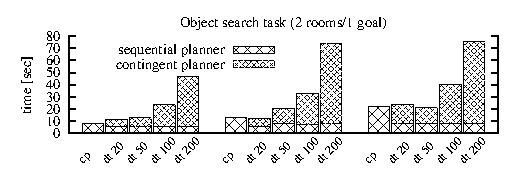
\includegraphics{dora1-time}\hfill
  % \vspace{2mm}
  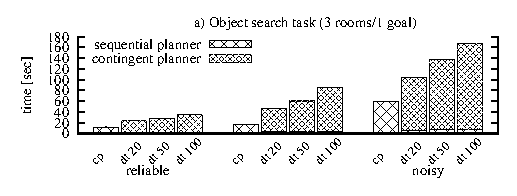
\includegraphics{dora2-time}\hfill
  % \vspace{2mm}
  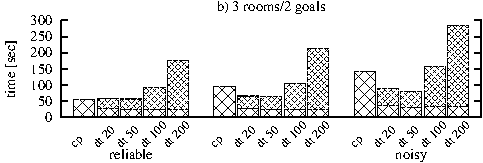
\includegraphics{dora3-time}\hfill
  % \vspace{2mm}
  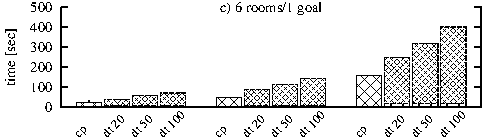
\includegraphics{dora4-time}\hfill
  \vspace{2mm}
  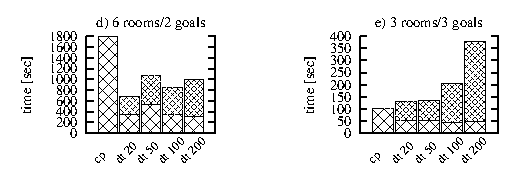
\includegraphics{dora56-time}\hfill
  \vspace{2mm}
  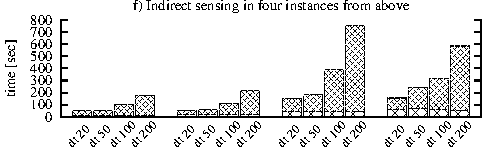
\includegraphics{dora-cat-time}\hfill
  \caption{Average runtime}
  \label{fig:results-time}
\end{figure}

\begin{figure}[h!]
  % \centering
  % 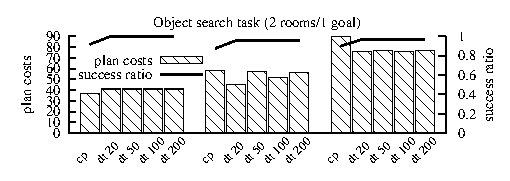
\includegraphics{dora1-quality}\hfill
  % \vspace{2mm}
  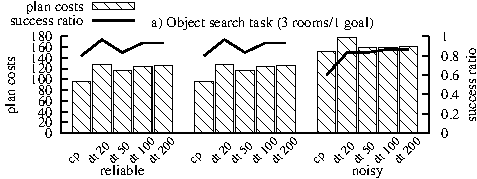
\includegraphics{dora2-quality}\hfill
  % \vspace{2mm}
  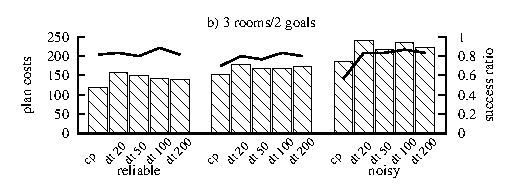
\includegraphics{dora3-quality}\hfill
  % \vspace{2mm}
  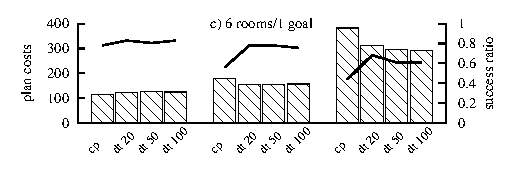
\includegraphics{dora4-quality}\hfill
  \vspace{2mm}
  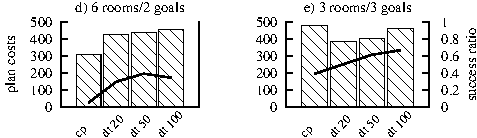
\includegraphics{dora56-quality}\hfill
  \vspace{2mm}
  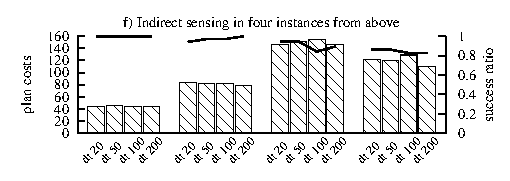
\includegraphics{dora-cat-quality}\hfill
  \caption{Average plan costs and number of successful runs.}
  \label{fig:results-quality}
\end{figure}


%% Figure \ref{fig:results-quality} shows the average costs of the
%% executed plans as well as the percentage of solvable tasks that were
%% actually solved by the planner. 

Examining success ratios and plan costs, where sensing is reliable
there is little to be gained by using the contingent planner, as the
greedy sensing approach of the baseline is sufficient. Not
surprisingly, as sensing degrades contingent planning pays off.  Also,
we find that time spent in contingent planning increases steeply as
the abstraction $\bstate_0$ becomes more refined.  That refinement
seems to be paying off in terms of the success ratio, particularly for
tasks $d$ and $e$, where we had sequential sessions using weighted
$A^*$ (rather than $A^*$). For less refined initial configurations,
the increase cost of contingent planning is compensated by a decrease
in Fast Downward planning times. The relatively high success rate
irrespective of the level of refinement in the initial configuration
indicates the effectiveness of using conditional entropy to guide
abstraction refinement in our setting.


%% :
%%while the resulting plans are still
%% longer on average, the impact on the number of solved tasks was much
%% smaller than for the baseline system.  

%% Less aggressive abstraction of the initial configuration results in
%% longer runtimes, with little to be gained in terms of plan quality. We
%% conclude that in our scenario it is worthwhile being assumptively
%% aggressive.  


%% \section{Discussion}
%% 

A theoretical criticism of switching continual planning, concerns
interleaved sequential and decision-theoretic sessions failing to make
any progress towards the objective.


\section{Related Work}
There have been a number of recent papers on
planning under uncertainty using systems that were intended for
sequential planning in deterministic problems,  for example,
\system{FFR$_a$}~\cite{yoon:etal:2007}, the winning entry from the
probabilistic track of the 2004 International Planning Competition.
In the continual paradigm, \system{FFR$_a$} uses the fast satisficing
procedure \system{FF}~\cite{hoffmann:nebel:2001} to compute sequential
plans and corresponding execution traces.
%%
More computationally expensive approaches in this vein combine
sampling strategies on valuations over {\em runtime variables} with
deterministic planning procedures. The outcome is typically a more
robust sequential plan~\cite{yoon:etal:2008}, or contingent
plan~\cite{majercik:2006}. 

%%No! They simply haven't been evaluated in PO settings. They may, or
%%may not struggle. They have sampling of traces, and that would
%%include observations, and therefore evolutions of beliefs. SSAT was
%%proposed by Littman for POMDPs. So the majercik stuff is perfectly
%%suited to POMDPs.

% Normally if we are going to compare with related work, we do
% actually *compare*. Why didn't you try those approaches? I think
% it's safe to say that FFR will struggle. Why would it even include
% in its plan an observational action that doesn't change the world?

%%
%% However, as we said in the introduction,
%% all these approaches struggle in partially observable domains as they
%% rely on being able to determine the state at all times.

Also leveraging deterministic planners in problems that feature
uncertainty, \system{Conformant-FF}~\cite{hoffmann:brafman:2006} and
$T_0$~\cite{palacios:geffner:2009} demonstrate how conformant planning
---i.e., sequential planning in unobservable worlds--- can be modelled
as a deterministic problem, and therefore solved using sequential
systems. In this conformant setting, advances have been towards
compact representations of beliefs amenable to existing best-first
search planning procedures, and lazy evaluations of beliefs. Most
recently this research thread has been extended to contingent planning
in fully observable non-deterministic
environments~\cite{albore:etal:2009}.
%%
The continual planning system that motivated our
project~\cite{brenner:nebel:jaamas09} also has this characteristic,
and has been applied in completely observable domains, particularly
those featuring multiple communicating agents. 

%% The use of knowledge
%% operators in domains allows plans that act to gain knowledge, but the
%% approach assumes that such actions are deterministic and reliable, an
%% assumption that we relax.

Our work is motivated by domains that contain a mixture of task
planning and observation planning. There have been a number of recent
papers representing observation planning problems as POMDPs and using
various techniques to manage the large state
space. \citeauthor{hippo-jnl}~(\citeyear{hippo-jnl}) take this
approach in a vision algorithm selection problem. In their case there
is a natural hierarchical decomposition of the problem which allows
them to solve large problems by breaking them into a set of small
POMDPs. \citeauthor{doshi08:pref_elic}~(\citeyear{doshi08:pref_elic})
represent a preference elicitation problem as a POMDP and take
advantage of symmetry in the belief space ---essentially the idea that
it does not matter what the value of the variable you are trying to
observe is--- to exponentially shrink the state space. Although we
have been actively exploring the \citeauthor{doshi08:pref_elic}
approach, we have yet to find those exploitable structures in our
domain due to the task planning requirement.



\section{Concluding Remarks}

From an automated planning perspective, the problem of practical
mobile robot control poses important and contrary challenges.
%%
On the one hand, planning and execution monitoring must be
lightweight, robust, timely, and should span the lifetime of the
robot. Those processes must seamlessly accommodate exogenous events,
changing objectives, and the underlying unpredictability of the
environment.
%%
On the other hand, robot planning should perform computationally
expensive reasoning about contingencies, and possible revisions of
subjective belief according to quantitatively modelled uncertainty in
acting and sensing. 

In this paper we address these challenges, developing a continual
planner that switches between fast sequential and expensive
decision-theoretic planning. Given a POMDP model of the environment,
sequential planning is used to compute an initial deterministic
sequential plan and complementary runtime evolution of the decision
process. That plan is executed until testing of an assumption about
the runtime state is scheduled. At that point a contingent session
performs some sensing which determines whether or not the sequential
session should be allowed to continue, or otherwise acts to achieve
the overall objectives.


The most pressing item for future research, is to develop a scheme
whereby the serial planner can relax {\em executability} assumptions,
so that conformant (or semi-conformant) plans can be executed without
interruption by a contingent session. A more general criticism of
switching continual planning concerns interleaved sequential and
contingent sessions failing to make any progress towards the
objectives. For example, in the worst case we can have each sequential
session producing an identical plan, and each decision-theoretic
session rejecting it without further sensing. Although this has not
been an issue in our work so far, it must be dealt with rigorously
in the future. We suggest that a good way to mitigate this problem is
by developing a {\em motivational} component that maintains a {\em
dynamic} reward model whose limiting behaviour prevents that switching
deadlock.





%% The sequential mode of our system always schedules decision-theoretic
%% planning before executing actions that are not applicable with
%% certainty. This is inefficient if the utility of the plan is not
%% dependent on that actions successful execution. This situation always
%% arises for conformant plans. 



%% The switching continual planning system we have described serves as
%% the underlying planner for CogX.




%% the effects of a {\em sense} schema are perceptual, whereas the
%% effects of an {\em operator} schema are over state propositions.




%% posted by a motivational component of the underlying robotic
%% architecture. 

%% contingent sensory plans that are tailored to current
%% objectives.

%% In this paper we present an approach to continual planning that uses
%% two planning systems. The first 
				   
%%  to a distinct class of
%% challenges. We suppose 
%% %%
%% The underlying environment is modelled as a POMDP. We use the fast
%% classical satisficing system FastDownward to find a deterministic
%% sequential plan and complementary runtime evolution of that
%% process. This corresponds to a generalisation of replanning in
%% probabilistic planning to problems with partial observability.

%% Interaction between the sequential planner and execution proceeds
%% more-or-less analogously to popular replanning approaches

%% Addressing these challenges in a monolithic framework, we present a
%% {\em switching} continual planner, that uses the fast sequential
%% satisficing procedure FastDownward to perform net-benefit
%% %%
%% makes reasonable assumptions about the evolution of the runtime state
%% given a POMDP model of the environment. 

%% contingent sensory plans that are tailored to current
%% objectives.


%% The decision-theoretic planner is able to tailor sensory processing on
%% a robot platform to the current objective, while FastDownward  quickly 


%% In this paper we develop a continual planing system that uses two
%% planning systems. The first, is a state-of-the-art domain independent
%% planner for deterministic problems. The second is a information-state
%% contingency planning the information-state space of 


%% Continual planning is a powerful technique that goes some way to
%% addressing those challenges. That approach interleaves planning and
%% execution, deliberately postponing planning for contingencies unless
%% they eventuate during execution. 


%% computing a single sequential plan and
%% eventuality



%% To these challenges it seems a continual planning approach is best, 

%% where the runtime state evolves during plan execution 


%% interleaved planning and execution. 

%% the latter is able to tailor sensory processing on a robot platform,
%% in order that it.

%% {\em ad-hoc} 

%% , reason about degrees of belief and uncertainty about the world, 

%% probabilistic sequential decision making in practical sized problems
%% is intractable.

%% quantitative probabilistic models of the perception and action .


%% The file named.bst is a bibliography style file for BibTeX 0.99c
\bibliographystyle{named}
\bibliography{ijcai11}

\end{document}

